% !TeX spellcheck = fr_FR
\chapter{Chapitre 7 : Résultats}
\label{chap:7}

\section{AED}
\label{sec:7.1}

\subsection{Entrainements pour différentes tailles de fenêtres}

\begin{table}[H]
	\centering{
		\begin{tabular}{c l c c}
			\hline
			\multicolumn{4}{c}{\textbf{AED}} \\
			\multicolumn{4}{c}{epochs = 50, $\eta$ = 0.005, nombre d'entrainements = 10} \\
			\hline
			\textbf{Nombre d'échantillons} & \textbf{Données} & \textbf{Valeur de perte moyenne} & \textbf{Ecart type} \\
			\hline
			\multirow{2}{*}{1024} & Entrainement & 0.0094 & 0.0038 \\
			& Validation & 0.0096 & 0.0076 \\
			\hline
			\multirow{2}{*}{2048} & Entrainement & 0.0096 & 0.0018 \\
			& Validation & 0.0083 & 0.0014 \\
			\hline
			\multirow{2}{*}{3072} & Entrainement & 0.0088 & 0.0025 \\
			& Validation & 0.0084 & 0.0014 \\
			\hline
			\multirow{2}{*}{4096} & Entrainement & 0.0089 & 0.0010 \\
			& Validation & 0.0085 & 0.0013 \\
			\hline
		\end{tabular}
		\caption[Entrainement de l'AED pour différentes tailles de fenêtres]{Entrainement de l'AED pour différentes tailles de fenêtres. Source : Réalisé par \textsc{Küenzi} Jean-Daniel}
		\label{tab:aed_training}
	}
\end{table}

Lorsqu'on observe ces résultats, on remarque que l'\gls{aed} a eu plus de peine à reconstruire les données non bruitées quand on utilise une fenêtre de 1024 échantillons. Cela peut être dû au fait que le bruit blanc gaussien ajouté est trop fort pour la taille de cette fenêtre. Toutefois, la valeur de perte moyenne reste assez faible et les données bruitées sont plutôt bien reconstruites sans le bruit. On remarque aussi qu'à partir d'une fenêtre de 2048 échantillons, l'augmentation du nombre d'échantillons ne fait pas augmenter cette valeur de perte, ce qui est positif, une valeur de perte plus grande veut dire une reconstruction des données moins bonne.

\subsection{Reconstruction d'une donnée non bruitée}

Dans cette partie, nous allons voir comment l'\gls{aed} se comporte lorsqu'il reçoit une donnée non bruitée en entrée. Pour cet exemple j'ai joué un A à 110 [Hz] avec le plectre.

\begin{figure}[H]
	\centering
	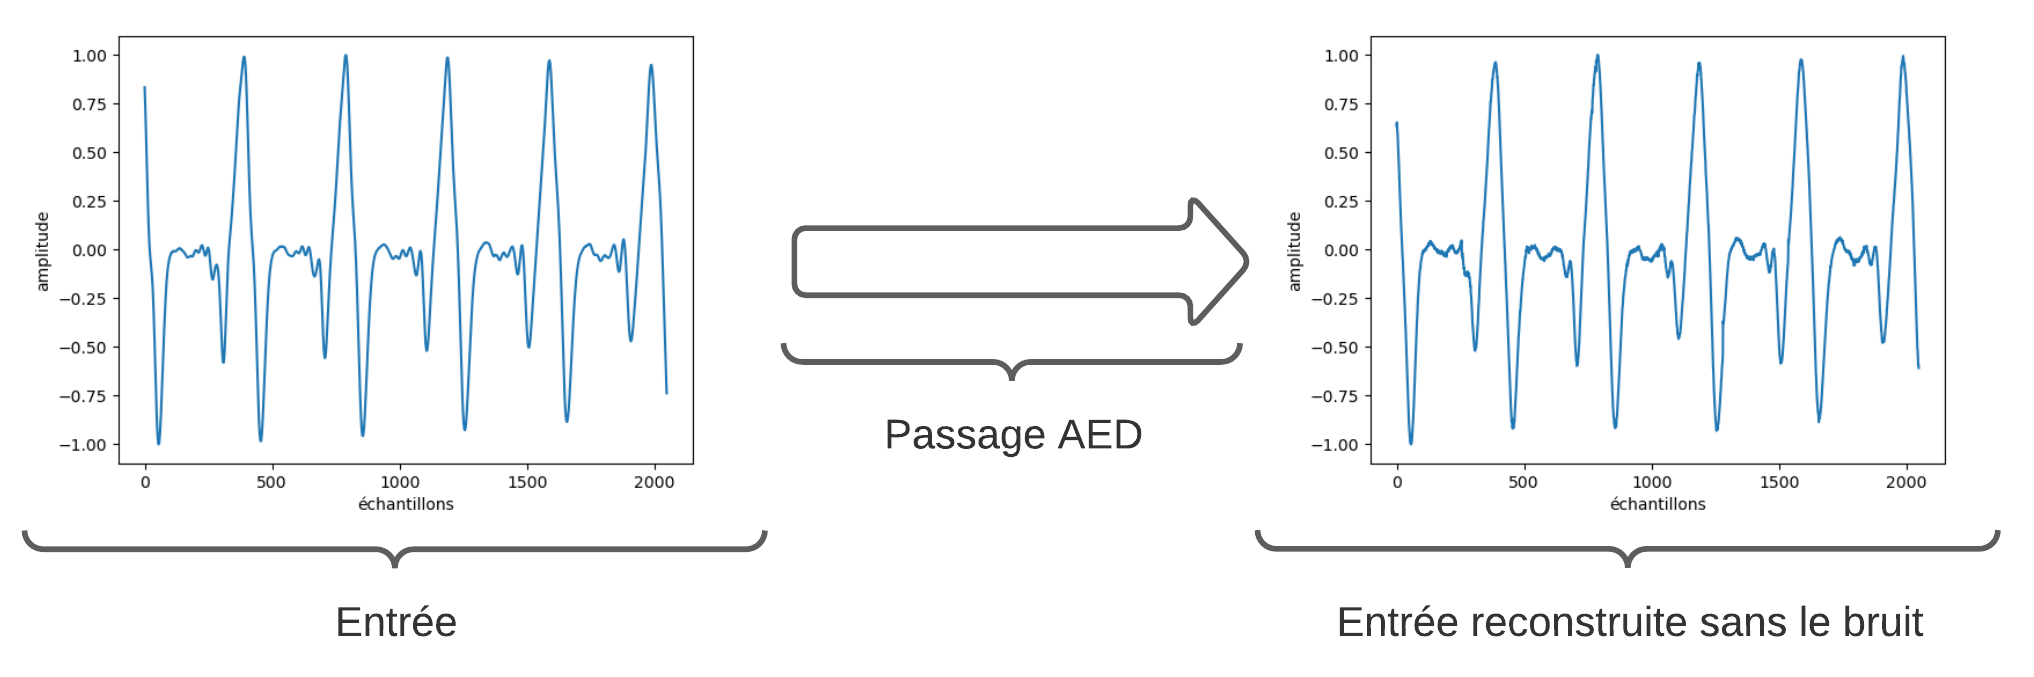
\includegraphics[width=1\linewidth]{aed_clean_denoise}
	\caption[Reconstruction d'un A à 110 Hertz non bruité]{Reconstruction d'un A à 110 [Hz] non bruité. Source : Réalisé par \textsc{Küenzi} Jean-Daniel}
	\label{fig:aed_clean_denoise}
\end{figure}

On peut constater que le signal à la sortie de l'\gls{aed} est quasiment le même qu'à l'entrée. Comme le signal d'entrée n'était pas bruité, l'\gls{aed} s'est uniquement contenté de reconstruire le même signal. On peut retrouver les différents pics du signal aux bons endroits, et l’on remarque entre chaque pic qu'il y a une très légère différence entre l'entrée et la sortie.

\subsection{Reconstruction d'une donnée avec du bruit blanc gaussien}

Dans cette partie, nous allons voir comment l'\gls{aed} se comporte lorsqu'il reçoit une donnée bruitée en entrée. Pour cet exemple, il s'agit du même A à 110 [Hz] de l'exemple précédent, mais avec du bruit blanc gaussien ajouté. Le bruit blanc gaussien qui a été ajouté a une moyenne de zéro et un écart type de zéro virgule trois. Ce bruit ajouté est comparable à un souffle constant assez fort.

\begin{figure}[H]
	\centering
	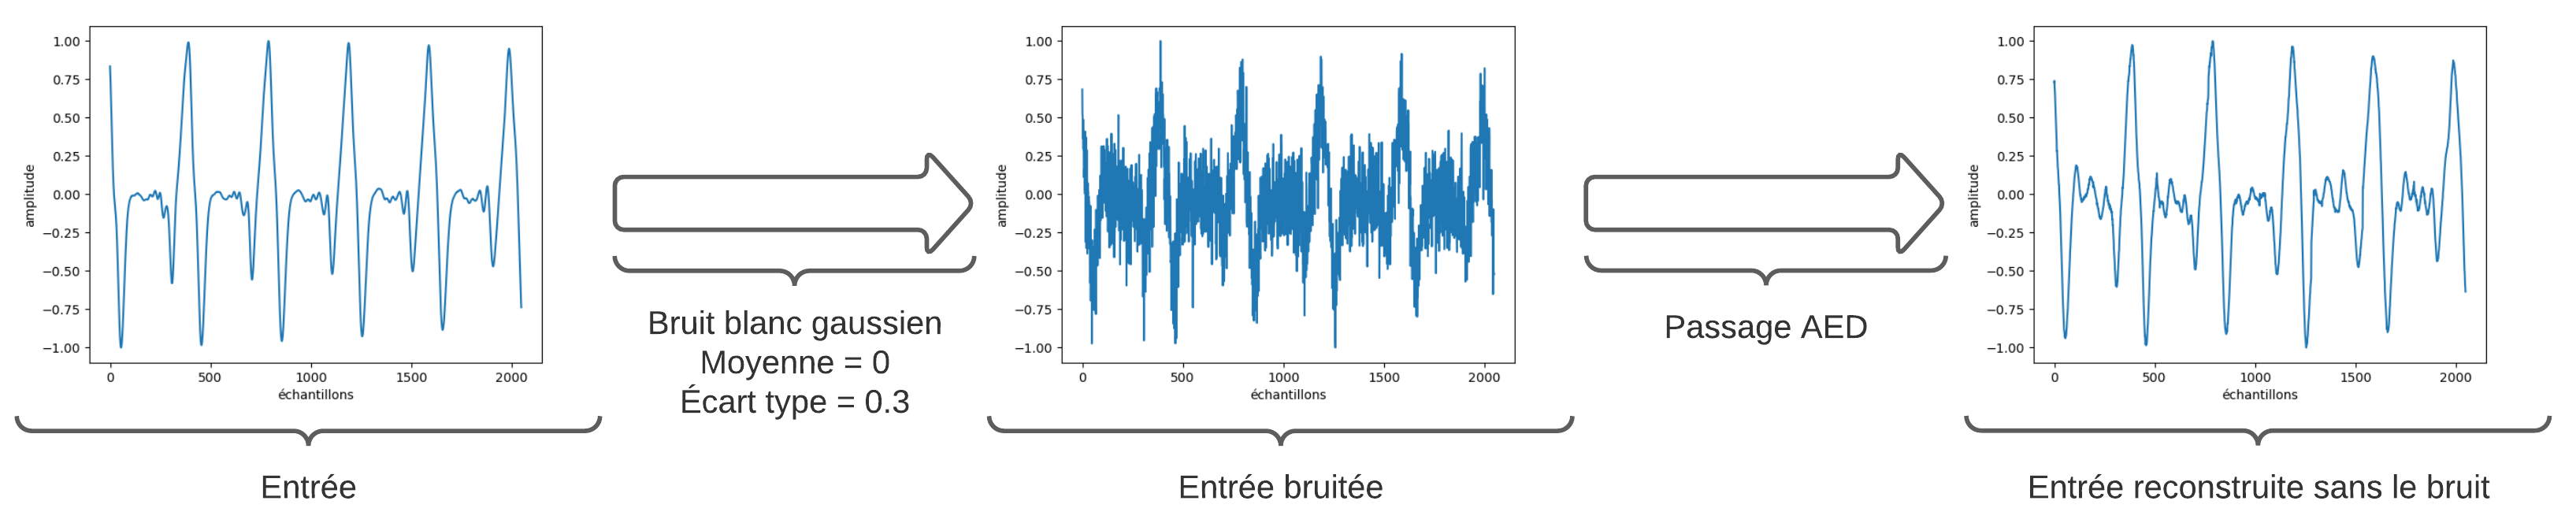
\includegraphics[width=1\linewidth]{aed_denoise}
	\caption[Reconstruction d'un A à 110 Hertz avec du bruit blanc gaussien]{Reconstruction d'un A à 110 [Hz] avec du bruit blanc gaussien. Source : Réalisé par \textsc{Küenzi} Jean-Daniel}
	\label{fig:aed_denoise}
\end{figure}

On peut constater que le signal à la sortie de l'\gls{aed} est semblable à celui qui est à l'entrée, mais légèrement différent. Comme le signal d'entrée était bruité, l'\gls{aed} à correctement extrait les caractéristiques nécessaires pour reconstruire le signal sans le bruit. On constate également que le signal reconstruit est quasiment le même que le signal qui se trouve en entrée. On peut retrouver les différents pics du signal aux bons endroits, et on remarque entre chaque pic, qu'il y a une différence entre l'entrée et la sortie.

\subsection{Reconstruction d'une donnée avec du gain}

Dans cette partie nous allons voir comment l'\gls{aed} se comporte lorsqu'il reçoit une donnée bruitée avec du gain en entrée. Pour cet exemple j'ai joué un Dmin avec la basse à \textasciitilde146,83[Hz]. Pour ajouter le gain dans le signal, j'ai utilisé un amplificateur \textsc{Aslin Dane AG-15R}. Toutefois, l'amplificateur étant assez vieux je n'ai pas réussi à trouver sa fiche technique et donc de ce fait, pas pu déterminer le gain ajouter en décibels.

\begin{figure}[H]
	\centering
	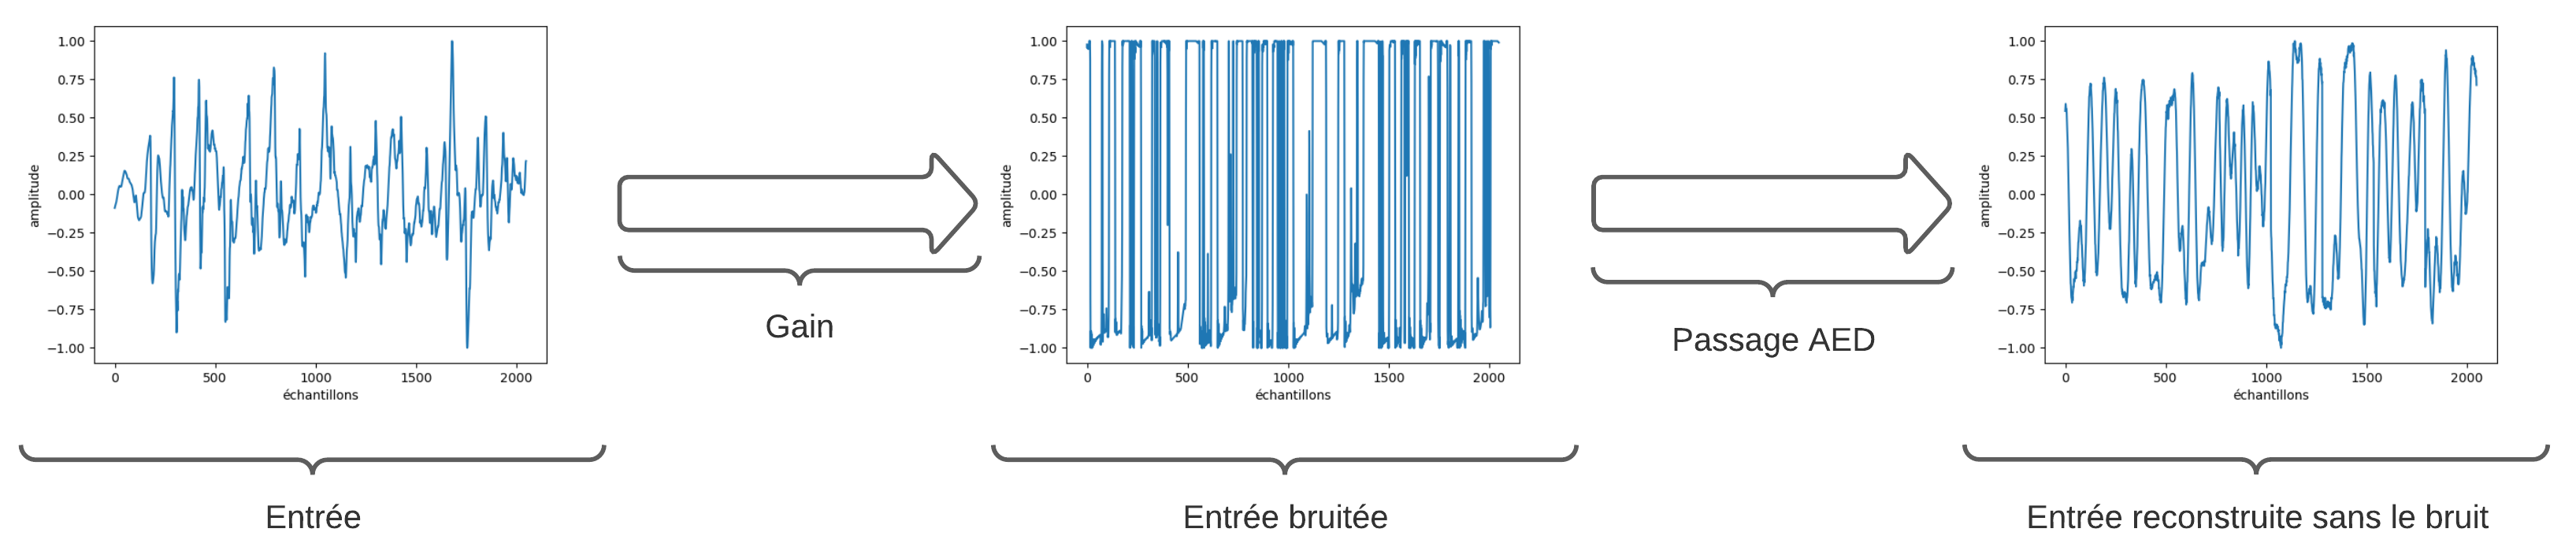
\includegraphics[width=1\linewidth]{aed_gain_denoise}
	\caption[Reconstruction d'un Dmin avec du gain]{Reconstruction d'un Dmin avec du gain. Source : Réalisé par \textsc{Küenzi} Jean-Daniel}
	\label{fig:aed_gain_denoise}
\end{figure}

On peut constater que le signal à la sortie de l'\gls{aed} est très différent de celui qui est en entrée. Cela est normal et compréhensible, l'\gls{aed} a été entrainé à reconstruire les données sans du bruit blanc gaussien et non pas à reconstruire les données sans du gain. De plus, on observe que le gain ajouté est vraiment fort et qu'il déforme énormément le signal, il en devient presque carré. Toutefois, on remarque que la reconstruction des données est assez intéressante,  l'\gls{aed} a réduit les amplitudes et rendu le signal moins carré. J'ai également observé que l'utilisation de l'\gls{aed} permettait au modèle de prédire beaucoup plus facilement l'accord avec du gain lors de l'utilisation en temps réel. Lorsque je n'utilisais pas l'\gls{aed} et que le modèle prenait le signal brut avec le gain, le modèle prédisait surtout la quinte et la tierce mais rarement l'accord. Avec l'\gls{aed}, il avait beaucoup plus de facilité à prédire l'accord.

\section{LSTMB}
\label{sec:7.2}

\subsection{Matrice de confusion sur l'ensemble de validation}

La matrice de confusion suivante a été réalisée avec le modèle utilisant une fenêtre de 2048 échantillons.

\begin{figure}[H]
	\centering
	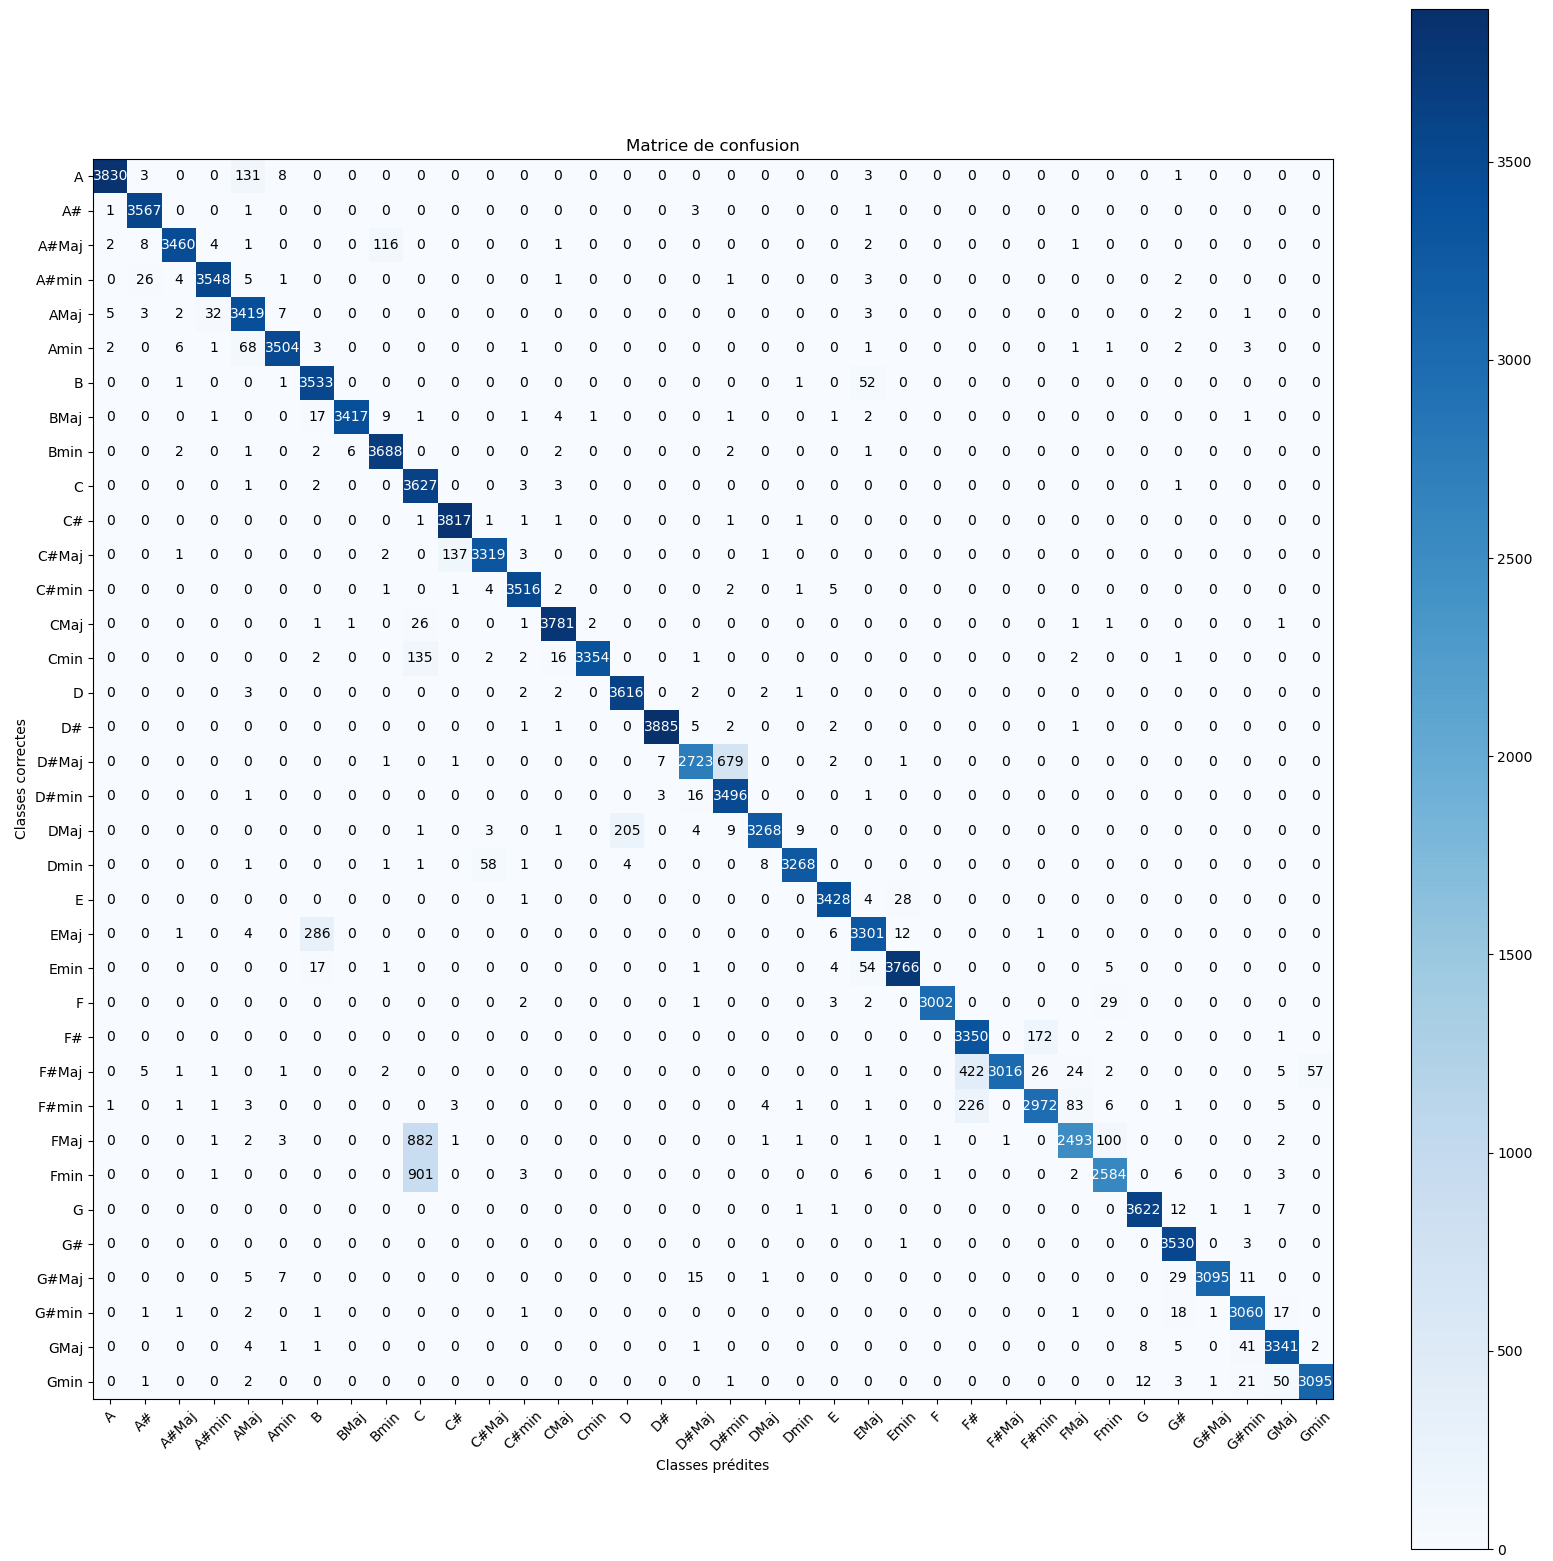
\includegraphics[width=1\linewidth]{cm_lstmb_fft}
	\caption[Matrice de confusion pour l'architecture LSTMB avec TFR]{Matrice de confusion pour l'architecture LSTMB avec TFR. Source : Réalisé par \textsc{Küenzi} Jean-Daniel}
	\label{fig:cm_lstmb_fft}
\end{figure}

Tout d'abord, lorsque l'on observe la matrice de confusion, on peut constater le même problème qui est décrit dans la \autoref{subsec:6.1.2} de la \autoref{sec:6.1}, c'est-à-dire que le modèle a prédit certaine composante des accords, comme la fondamentale, la tierce ou la quinte. En fait cela n'est pas réellement une erreur et relève plutôt d'une imperfection dans l'ensemble de validation. Aussi on remarque que la grande majorité des données sont correctement classées (visible par la diagonale qui traverse la matrice). Toutefois, le modèle confond parfois les accords majeurs et mineurs. 

Ainsi, comme décrit dans la \autoref{subsec:6.2.2} de la \autoref{sec:6.2}, il confond les accords qui sont assez proches. C'est notamment le cas avec A\sh Maj que le modèle a confondu avec un Bmin. Finalement les résultats de l'architecture \gls{lstmb} avec \gls{tfr} sont très similaires aux résultats obtenus avec l'architecture \gls{pmc} avec \gls{tfr} et sont dans leurs globalités excellents.

\subsection{Entrainements pour différentes tailles de fenêtres}

\begin{table}[H]
	\centering{
		\begin{tabular}{c l c c}
			\hline
			\multicolumn{4}{c}{\textbf{LSTMB avec \gls{tfr}}} \\
			\multicolumn{4}{c}{epochs = 50, $\eta$ = 0.005, nombre d'entrainements = 10} \\
			\hline
			\textbf{Nombre d'échantillons} & \textbf{Données} & \textbf{Précision moyenne \%} & \textbf{Ecart type \%} \\
			\hline
			\multirow{2}{*}{1024} & Entrainement & 99.53 & 0.11 \\
			& Validation & 85.32 & 0.45 \\
			\hline
			\multirow{2}{*}{2048} & Entrainement & 99.81 & 0.01 \\
			& Validation & 95.51 & 0.33 \\
			\hline
			\multirow{2}{*}{3072} & Entrainement & 99.88 & 0.02 \\
			& Validation & 94.88 & 0.23 \\
			\hline
			\multirow{2}{*}{4096} & Entrainement & 99.91 & 0.01 \\
			& Validation & 94.30 & 0.26 \\
			\hline
		\end{tabular}
		\caption[Entrainement de l'architecture LSTMB avec TFR]{Entrainement de l'architecture LSTMB avec TFR. Source : Réalisé par \textsc{Küenzi} Jean-Daniel}
		\label{tab:lstm_with_tfr}
	}
\end{table}

Lorsque l'on observe ces résultats, le premier constat est le même que pour l'architecture \gls{pmc} et \gls{rnc} avec \gls{tfr}. Une fenêtre de 1024 échantillons n'est pas suffisante pour permettre une bonne prédiction des classes. Avec 1024 échantillons, nous avons une résolution fréquentielle de \textasciitilde$43.06$[Hz]. Nous ne sommes donc pas du tout précis et cela va fortement impacter le modèle lors de la prédiction. Ensuite, on remarque que l'architecture \gls{lstmb} avec \gls{tfr} nous a donné les meilleurs résultats avec une fenêtre de 2048 échantillons. Comme précisé dans la \autoref{sec:3.7}, les cellules \gls{lstm} sont très efficaces dans le traitement de données chronologiques. Finalement, on remarque qu'à partir de la fenêtre avec 2048 échantillons, augmenter le nombre d'échantillons fait chuter la précision. Cela peut être en partie dû à la réduction de la taille de l'ensemble de données ainsi qu'au problème évoqué dans la \autoref{subsec:6.1.2}. 

\begin{table}[H]
	\centering{
		\begin{tabular}{c l c c}
			\hline
			\multicolumn{4}{c}{\textbf{LSTMB sans \gls{tfr}}} \\
			\multicolumn{4}{c}{epochs = 50, $\eta$ = 0.005, nombre d'entrainements = 10} \\
			\hline
			\textbf{Nombre d'échantillons} & \textbf{Données} & \textbf{Précision moyenne \%} & \textbf{Ecart type \%} \\
			\hline
			\multirow{2}{*}{1024} & Entrainement & 99.69 & 0.15 \\
			& Validation & 91.49 & 0.22 \\
			\hline
			\multirow{2}{*}{2048} & Entrainement & 99.91 & 0.02 \\
			& Validation & 92.45 & 0.54 \\
			\hline
			\multirow{2}{*}{3072} & Entrainement & 99.94 & 0.05 \\
			& Validation & 92.21 & 0.15 \\
			\hline
			\multirow{2}{*}{4096} & Entrainement & 99.94 & 0.03 \\
			& Validation & 91.25 & 0.16 \\
			\hline
		\end{tabular}
		\caption[Entrainement de l'architecture LSTMB sans TFR]{Entrainement de l'architecture LSTMB sans TFR. Source : Réalisé par \textsc{Küenzi} Jean-Daniel}
		\label{tab:lstm_without_tfr}
	}
\end{table}

En observant ces résultats, on constate tout d'abord qu'ils sont légèrement moins bons que ceux de l'architecture avec \gls{tfr}, mais l'on remarque aussi que la fenêtre de 2048 échantillons donne le meilleur résultat entre les trois architectures sans \gls{tfr}. Néanmoins, ces résultats sont très encourageants, on remarque que le modèle a une assez bonne précision avec les données discrètes. On remarque également qu'à partir de la fenêtre avec 2048 échantillons, l'augmentation du nombre d'échantillons fait légèrement chuter la précision du modèle. Cela peut être dû au nombre d'epochs qui n'est plus suffisant pour laisser au réseau le temps de bien converger ou à la réduction de la taille de l'ensemble de données ainsi qu'au problème évoqué dans la \autoref{subsec:6.1.2}.

\section{Ressenti d'utilisation en temps réel}
\label{sec:7.3}

Lors de mon utilisation en temps réel, j'ai tout d'abord constaté que les accords et notes joués étaient correctement prédits. De plus, j'ai mesuré le temps passé à traverser le modèle, avec une utilisation en CPU, depuis le moment où nous avons nos 2048 échantillons jusqu'à l'obtention de la prédiction de l'accord ou de la note. En moyenne, cela prend entre trois et quatre millisecondes, nous sommes donc bien en dessous des cinq millisecondes visées. De plus, lors de l'utilisation en temps réel le modèle prend en entrée une fenêtre de 2048 échantillons, ce qui représente une durée de \textasciitilde$0.046$[s]. Mais j'utilise une taille de chevauchement de 1024 échantillons, soit \textasciitilde$0.023$[s], ce qui fait que la toutes premières fenêtre aura une latence de \textasciitilde$0.046$[s], mais les autres fenêtres auront une latence divisée par un facteur de deux grâce au chevauchement, soit une latence de \textasciitilde$0.023$[s]. En somme, on utilise les 1024 derniers échantillons de la fenêtre à l'instant $t-1$ pour construire notre fenêtre à l'instant $t$. La latence visuelle est donc presque imperceptible et l'impression du temps réel se fait bien ressentir.

Ensuite, concernant l'attaque, elle est légèrement visible au début de la prédiction, c'est-à-dire lors de la première fenêtre. Elle est donc uniquement visible pendant \textasciitilde$0.046$[s] ce qui n'est pas très gênant.

J'ai également constaté que le modèle ne semble pas avoir de problèmes avec les changements de phases dans les signaux. J'ai notamment testé différentes techniques de legato (hammer-on, pull-off, etc.), c'est-à-dire que j'ai lié les notes jouées sans laisser de silence entre elles et sans réattaquer la corde avec le plectre ou le doigt. Ce qui est intéressant avec ces techniques, c'est qu'elles vont créer un changement de phase brusque dans le signal, étant donné que l'on va par exemple passer d'un F à un F\sh\,ou un G de manière instantanée.

J'ai aussi testé différends bends (technique à la guitare), c'est-à-dire que j'ai volontairement tiré latéralement la corde sur laquelle je jouais pour augmenter sa vibration et ainsi atteindre une note différente (par exemple pour atteindre un G depuis un F). Cette technique est très intéressante, car elle nous fait passer par toutes les fréquences entre la note de base et la note visée. Par exemple pour passer d'un F à un G dans la même octave, nous allons passer par toutes la bande de fréquence [174.61; 196.00]. C'est donc un bon moyen de déterminer si le modèle est sensible aux changements de phases.

J'ai constaté de plus que le modèle a plus de facilité à détecter les notes que les accords, ce qui est compréhensible étant donné que le spectre de Fourier d'une note, et donc d'un signal, est beaucoup moins complexe que celui d'un accord qui est une agrégation de plusieurs notes, et donc signaux différents.

Pour finir, j'ai rajouté la fondamentale et la quinte plusieurs fois à l'octave dans l'accord et donc de ne plus jouer un accord à trois sons, comme au départ, mais de jouer un accord avec six sons. Par exemple l'accord EMaj est joué avec les notes dans l'ordre suivant :

\begin{table}[H]
	\centering{
		\begin{tabular}{|l|c|c|c|}
			\hline
			\multicolumn{4}{|c|}{\textbf{A Majeur}} \\
			\hline
			& \textbf{Notes} & \textbf{Octave} & \textbf{Fréquence en [Hz]} \\
			\hline
			Fondamentale & E & 1 & 82.41 \\
			\hline
			Quinte juste & B & 1 & 123.47 \\
			\hline
			Fondamentale & E & 2 & 164.81 \\
			\hline
			Tierce majeure & G\sh & 2 & 207.65 \\
			\hline
			Quinte & B & 2 & 246.94 \\
			\hline
			Fondamentale & E & 3 & 329.63 \\
			\hline 
		\end{tabular}
		\caption[Accord AMaj avec la quinte et la fondamentale sur plusieurs octaves]{Accord AMaj avec la quinte et la fondamentale sur plusieurs octaves. Source : Réalisé par \textsc{Küenzi} Jean-Daniel. A partir de \textit{Wikipedia}, ref. URL11}
		\label{tab:full_amaj}
	}
\end{table}

Le fait de rajouter des composantes comme la fondamentale et la quinte à l'octave ne gêne pas les prédictions du modèle et cela peut s'expliquer par le fait que sur le spectre de Fourier, nous allons retrouver les trois composantes de l'accord à trois sons, à savoir la fondamentale, la tierce et la quinte juste. De plus, comme les composantes rajoutées sont des multiples des trois composantes de bases, cela correspond donc aux partiels harmoniques qui étaient déjà présents sur le spectre, mais cette fois elles seront plus fortes et vont à leurs tours rajouter leur propre partiels harmoniques.
